%!TEX root = ../main.tex

\chapter{Python}

Die Entwicklung von Python begann 1991 unter der Leitung von Guido van Rossum. Seine Ziele lagen darin, eine Sprache zu entwickeln, die einfach und intuitiv ist, deren Quelltext sich so einfach liest wie reines Englisch, die alltägliche Aufgaben mit geringer Entwicklungszeit lösen kann und Open Source sein soll.
Laut der Entwicklerumfrage von Stack Overflow wird Python jedes Jahr beliebter. 2019 überholte Python die Programmiersprache Java auf der Rangliste der beliebtesten Programmiersprachen. 

\begin{figure}[!htb]
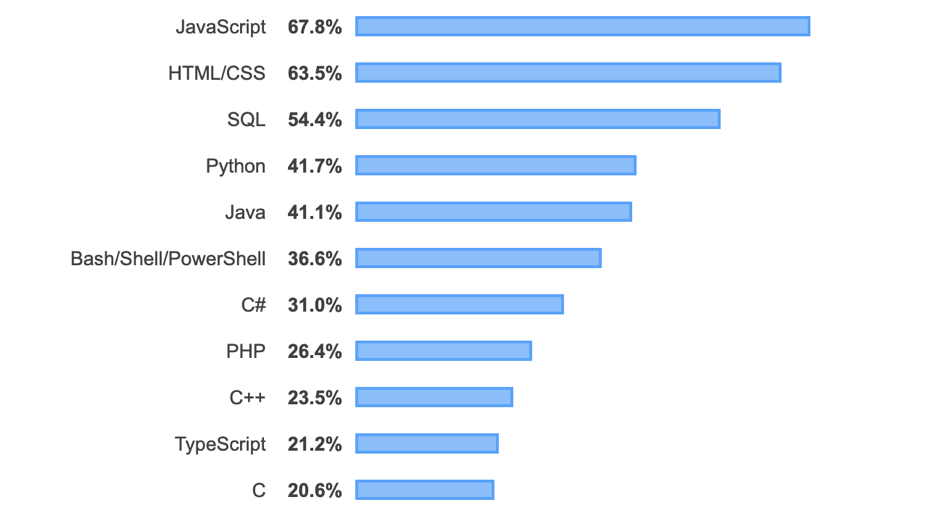
\includegraphics{stackOverflow.png}%
\caption{Rangliste der beliebtesten Programmiersprachen }
\label{img:stackoverflowBild}
\end{figure}

25\% der Entwickler, die noch nicht mit Python gearbeitet haben, möchten diese Sprache gerne lernen. Diese Lernbereitschaft wurde in den letzten drei Jahren von keiner anderen Programmiersprache überboten \cite{stackoverflow}. Das spricht sehr dafür, dass Python in den kommenden Jahren immer weiter an Bedeutung gewinnen wird. In dieser wissenschaftlichen Ausarbeitung wurde Python verwendet, um einige der Graphen und Kennlinien zu erzeugen. 

\section{Objektorientierte Programmierung in Python}

Im folgendem wird die objektorientierte Programmierung in Python anhand der vier Grundprinzipien, Generalisierung, Vererbung, Kapselung und Polymorphismus erläutert. 

\subsection{Klasse}

Zu den grundliegenden Bausteinen der objektorientierten Programmierung gehören die Klassen. Mithilfe einer Klasse lassen sich eigenen Datentypen definieren. Ein anschauliches Beispiel hierfür ist die Adresse. Die Adresse besteht aus den Strings - Straßenname und Ort und aus den integer Werten - Hausnummer und Postleitzahl. Die einzelnen Datentypen können nun in einer eigenen Klasse names Adresse gesammelt werden. Die Variablen einer Klasse bezeichnet man als Instanzvariablen. 
Instanzvariablen besitzen zugriffsrechte. Nach dem prinzip des data hiding vergeben wir private Zugriffsrechte, das bedeutet das die Instanzvariablen nur innerhalb der Klasse bekannt sind und beeinflusst werden können.
Neben Instanzvariablen können Klassen auch Methoden besitzten. Methoden können die Instanzvariablen auslesen und beeinflussen. Grundlegende Methoden sind zum Beispiel \texttt{getter} und \texttt{setter}. Werden diese Methoden implementiert, können die privaten Zugriffsrechte umgangen werden. Durch die \texttt{setter} Methoden erhält man Schreibrechte und durch die \texttt{getter} Methoden Leserechte \cite{JavaRatz}.
Instanzvariablen, Zugriffsrechte und Methoden einer Klasse lassen sich anschaulich in einem UML Klassendiagrammen darstellen. In Abbildung \ref{img:AdresseUML} ist das UML Klassendiagramm der Klasse Adresse mit seinen \texttt{getter} und \texttt{setter} Methoden und Instanzvariablen dargestellt. 

\begin{figure}[!htb]
    \centering
    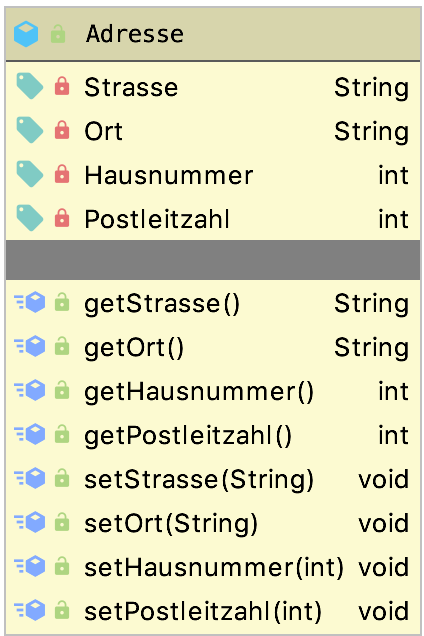
\includegraphics[scale=0.5]{AdresseUML.png}
    \caption{Die Klasse Adresse mit getter und setter Methoden}
    \label{img:AdresseUML}
\end{figure}

Um den neu definierten Datentyp zu nutzen, erzeugen wir Objekte der Klasse. Wir weisen dafür den Instanzvariablen konkrete Werte zu. Sowohl in Java als auch in Python nutzt man für die Instanziierung von Objekten eine Methode, die Konstruktor \footnote{In Python  Initialisierungsmethode} genannt wird . Der Konstruktor ist vergleichbar mit der \texttt{set} Methode. Beim aufrufen des Konstruktors übergibt man ihm die konkreten Werte der Instanzvariablen und erhält als rückgabewert eine Referenz auf das erzeugte Objekt. Die folgenden Codebeispiele zeigen die Implementierung der Klasse Adresse in Java \ref{Adressejava} und Python \ref{AdressePython}.

%Code Beispiele für die Klasse Adresse in Java und Python.
\begin{lstlisting}[caption=Die Klasse Adresse in Java, label=Adressejava]
public class Adresse
{
    //Instanzvariablen
    private String Strasse;
    private String Ort;
    private int Hausnummer;
    private int Postleitzahl;

    //Konstruktor
    public Adresse(String strasse, String ort, int hausnummer, int postleitzahl)
    {
        this.Strasse = strasse;
        this.Ort = ort;
        this.Hausnummer = hausnummer;
        this.Postleitzahl = postleitzahl;
    }

    //get Methode
    public String getStrasse() 
    {
        return Strasse;
    }

    //set Methode
    public void setStrasse (String strasse)
    {
        this.Strasse = strasse;
    }
}
\end{lstlisting}

\begin{lstlisting}[caption=Die Klasse Adresse in Python, label=AdressePython,language=Python]
class Adresse:
    #Initialisierungsmethode (Konstruktor)
    def __init__(self,strasse: str, hausnummer: int, postleitzahl: int, ort: str) -> None:
        self._strasse = strasse
        self._hausnummer = hausnummer
        self._postleitzahl = postleitzahl
        self._ort = ort   

    #get Methode
    def getStrasse(self) -> str:
        return self._strasse

    #set Methode
    def setStrasse(self, strasse: str) -> None:
        self._strasse = strasse

\end{lstlisting}

Der wohl auffälligste Unterschied bei der Implementierung der Klasse Adresse liegt bei den Instanzvariablen. In Java werden die Instanzvariablen einzeln mit ihren Zugriffsrechten und Datentypen angegeben. Für Python wird das nicht benötigt. Die Zugriffsrechte der Instanzvariablen von Python werden nicht durch Schlüsselwörter wie \texttt{private} festgelegt, sondern durch ein Unterstrich. Hierbei handelt es sich um eine Namenskonvention. Der Unterstrich vor dem Namen der Variable signalisiert dem Programmierer, das diese Instanzvariable als privat betrachtet werden soll. Sie hindert den Programmierer aber nicht daran auf die Variable zu zugreifen und zu verändern. In Python gilt die Philosophie, das der direkte Zugriff auf Attribute erlaubt und gewünscht ist \cite{PythonKalista}. Desweiteren ist die Datentyp Annotation des Rückgabewertes \footnote{def Methodenname() \textbf{\texttt{-> str}}} und der Methodenparameter in Python optional \cite{PythonBarry}. 


\subsection{Generalisierung}

\subsection{Vererbung}
\subsection{Kapselung}
\subsection{Polymorphismus}


